\documentclass[9pt]{beamer}

\usepackage[utf8x]{inputenc}

\usetheme{Ampang}
%\usecolortheme{ampangcolor}
%\usecolortheme{warna}

%%% XeLaTeX engine for Ubuntu Font support
\usepackage{xltxtra}
\setsansfont[
BoldFont=Ubuntu-Bold.ttf,
ItalicFont=Ubuntu-Italic.ttf,
BoldItalicFont=Ubuntu-BoldItalic.ttf
]
{Ubuntu-Regular.ttf}
\setmonofont{UbuntuMono-Regular.ttf}


\title{ROPER:\\A Genetic ROP-Chain Compiler Targetting Embedded Devices}
\author{Olivia Lucca Fraser}
\date{June - August, 2016}
\institute{NIMS Lab, Dalhousie University}

\begin{document}

\maketitle


\section{Genetic Algorithms}

\begin{frame}{0.0 There are Approximately 7 ARM Processors on the Market for Every Living Human}

\includegraphics[width=\textwidth]{internet-of-things-transparent.png}

ARM is now the de facto standard architecture for embedded and mobile devices, including phones, routers, pacemakers, surveillance cameras, printers, tablets, cars, etc.
\end{frame}

\begin{frame}{0.1 Return Oriented Programming (ROP-chain attacks)}
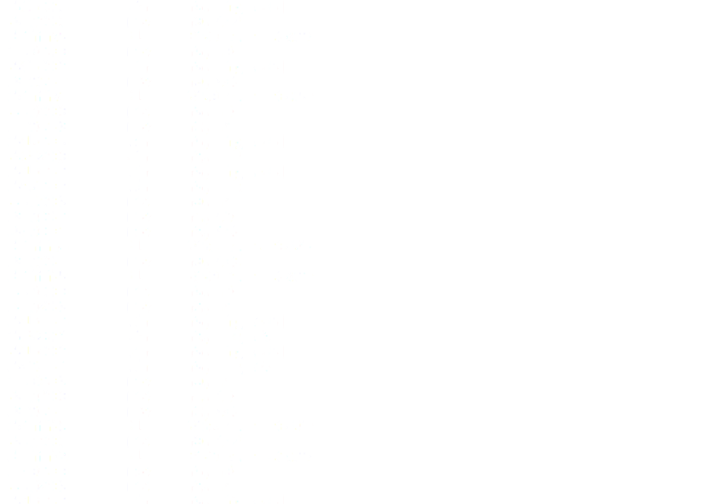
\includegraphics[width=\textwidth]{rop-chain-diagram.png}
\end{frame}



\begin{frame}{0.2 Return-Oriented Programming, cont.}

\begin{itemize}
\item If we can't write shellcode to executable memory, then we'll just have to make use of memory that has \emph{already} been marked executable.
\item This means salvaging whatever `gadgets' we can find there and using them to build our payload.
\end{itemize}
 

\begin{columns}

\begin{column}{0.3\textwidth}

\includegraphics[width=1.1\textwidth]{macgyver-transparent.png}
\end{column}


\begin{column}{0.7\textwidth}
\small

\begin{itemize}

\item any chunk of code sitting in executable memory can act as a gadget so long as we can regain control of programme after it executed

\item typically this means that gadgets end with a ``return'' instruction

\item hence the term ``Return Oriented Programming''

\item gadgets can be chained together to form arbitrarily complex programmes

\item typically they are implemented as stacks of addresses, each pointing to a gadget that ends by hopping to the next address in the stack

\item building these chains manually is difficult

%\item the easiest way to implement this is as a stack of addresses, which each point to a gadget that ends with an instruction to pop the stack into the instruction pointer
% \item a gadget is just a series of machine instructions that ends with a `return' instruction -- it is a generalization of the concept of subroutine or function;
% \item a return instruction is any instruction that restores instruction pointer from a definite storage location, typically so that execution can be resumed after the subroutine is complete;
% \item the return address is typically fetched either from the stack or from a special register;
% \item if we can write to the stack, we can control the flow of execution by supplying our own series of ``return addresses'';
% \item gadgets can be chained together into arbitrarily complex programmes, but this takes a MacGyver-like knack for working with found objects.

\end{itemize}


\end{column}

\end{columns}
    
\end{frame}

\begin{frame}{0.3 Genetic Algorithms: Natural Selection in Code}
  \begin{center}
    
\includegraphics[width=0.65\textwidth]{AI_ooze_transparent.png}
    \end{center}
  \begin{columns}
  
  \begin{column}{0.5\textwidth}

Natural selection can be implemented in code. 

We just need the space of possible solutions to exhibit:
  \begin{itemize}
  \item \textbf{variation} (sexual recombination or mutation, e.g.)
  \item \textbf{inheritance} (trivial, since we can copy code freely)
  \item \textbf{selection} (with respect to a fitness function)
  \end{itemize}
  
%   The basic idea is that Darwinian natural selection is an algorithm that can be specified in an entirely abstract fashion, and which can be implemented in code no less than in the organic world. 
  
%   \ \ \ \ Given a well-defined problem, with a few very general characteristics, we can use GA to \emph{evolve} a solution. 
  
  \end{column}
  
  \begin{column}{0.5\textwidth}
    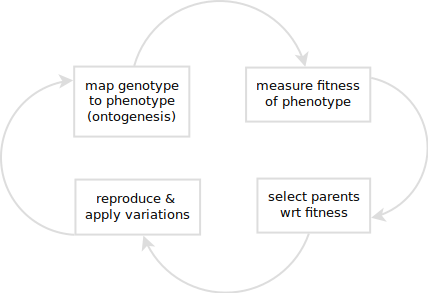
\includegraphics[width=\textwidth]{ga.png}
  %%% short explanation of what genetic algorithms are.

  
  \end{column}
  \end{columns}

   

\end{frame}


\begin{frame}{0.4 Genetic Algorithms in Offensive Security}

    There has been surprisingly little usage of evolutionary methods in offensive security, as far as I'm aware. Some notable exceptions include:
    
    \begin{itemize}
    
    \item At DEFCON 21 (2013), Soen Vanned presented a tool that used GA to fuzz web forms over HTTP/HTTPS and test for vulnerabilities to SQL and shell command injection.
    
    \item Genetic algorithms have also been put to good use in code fuzzing (auditing a code base for bugs and vulnerabilities). The most prominent example is American Fuzzy Lop, developed by Michal Zalewski (AKA lcamtuf). 
    
    
    \item 2006-2009 in the \textbf{NIMS} lab: Gunes Kayacik conducted a series of experiments, using genetic algorithms to develop stack-overflow shellcode attacks against Unix utilities, aiming to evade adaptive intrusion detection systems by training the attacks to mimic `normal' behaviour.
    
    \end{itemize}

\end{frame}

\begin{frame}{0.5 Question}%{The question:}
 \huge \textbf{Can we utilize genetic algorithms to \emph{evolve} ROP-chain payloads out of the ``primordial ooze'' of executable memory?}
 
% Can we automate MacGyver?
\end{frame}

%%%%%%%%%%%%%%%%%%%%%%%%%%%%%%%%%%%%%%%%%%%%%%%%%%%%%%%
\section{ROP-chain Attacks}

% \begin{frame}{Obsolescence of Traditional Shellcode Attacks}

% \begin{itemize}
%     \item Kayacik's experiments were successful\dots
%     \item but the form of attack he studied is no longer viable. 
% \end{itemize}


% \begin{columns}

% \begin{column}{0.3\textwidth}
% % some art
% 
\includegraphics[width=0.9\textwidth]{mario-jump-transparent.png}
% \end{column}

% \begin{column}{0.7\textwidth}

% \begin{itemize}
%     \item \textbf{Software defences} (DEP/NX): Compilers nowadays will usually map process's writeable memory as non-executable, and vice versa. 
    
%     \item \textbf{Hardware defences}: many processors nowadays (such as the ARM) physically separate code and data pipelines.
% \end{itemize}
% \end{column}

% \end{columns}

% \end{frame}

%%%%%%%%%%%%%%%%%%%%%%%%%%%%%%%%%%%%%%%%%%%%%%%%%%%%%%%



% \begin{frame}{The ARM Processor: A Ubiquitous and Challenging Target for ROP Attacks}
% \vspace{0.5cm}

% \begin{itemize}
% \item possibly the most common processor currently in use
% \item sold in almost 200 countries
% \item ARM processors outnumber humans by a factor of 7
% \item the de facto standard for phones, tablets, routers, ``the Internet of Things'', etc.

% \end{itemize}
% % This form of attack is particularly useful against systems using ARM processors, which are extremely common in embedded and mobile devices (phones, tablets, routers, `The Internet of Things', etc.). The ARM processor is today nearly ubiquitous; they are available in almost 200 countries, and outnumber humans by a factor of seven. 

% %\vspace{0.5cm}

% \begin{columns}
% \begin{column}{0.25\textwidth}
% [[ PUT DIAGRAM HERE ]]
% \end{column}

% \begin{column}{0.75\textwidth}
% \begin{itemize}
% \normal

% \item ARM processors nowadays employ a Harvard as opposed to a Von Neumann architectures -- the instruction and data pipelines are physically separated, blocking traditional shellcode attacks

% %\item this makes it much more difficult to find memory that be both written to \emph{and} executed by the attacker;

% \item ARM can alternate between two different instruction modes: ARM mode, which uses 32-bit instructions, and Thumb mode, where instructions are mostly 16 bits long

% \item the same stretch of memory can be parsed either way, affording us many more potential gadgets 

% \end{itemize}
% \end{column}


% \end{columns}



% \end{frame}



\begin{frame}{0.6 Introducing ROPER: A genetic engine for the evolution of ROP-chain payloads, targeting the ARM processor}

\textbf{Genotype:} a stack of addresses that can be derefrenced into ROP-gadgets. 
\vspace{10pt}

\textbf{Phenotype:} the behaviour of the CPU when this stack is executed (when it is popped into the program counter register).

\begin{columns}

    \begin{column}{0.3\textwidth}
    
\includegraphics[width=4cm]{inverted-transparent-roper.png}
    \end{column}
    \begin{column}{0.7\textwidth}
    
    \begin{itemize}
    \item ROPER analyses target ELF binary file, and extracts ROP gadgets;
    \item these act as a \textbf{``gene pool''} out of which a random population of ROP-chains is initialized;
    \item each generation, a sample of chains are evaluated in a \textbf{virtual environment},
    \item we isolate the \textbf{``fittest''} chains, the ones that come closest to bringing about the desired CPU context,
    \item and encourage them to \textbf{breed} and \textbf{mutate},
    \item until they \textbf{converge} on a chain that accomplishes the task in question.
    \end{itemize}
    
    \end{column}
\end{columns}
\end{frame}

\begin{frame}{0.7 How ROPER works}


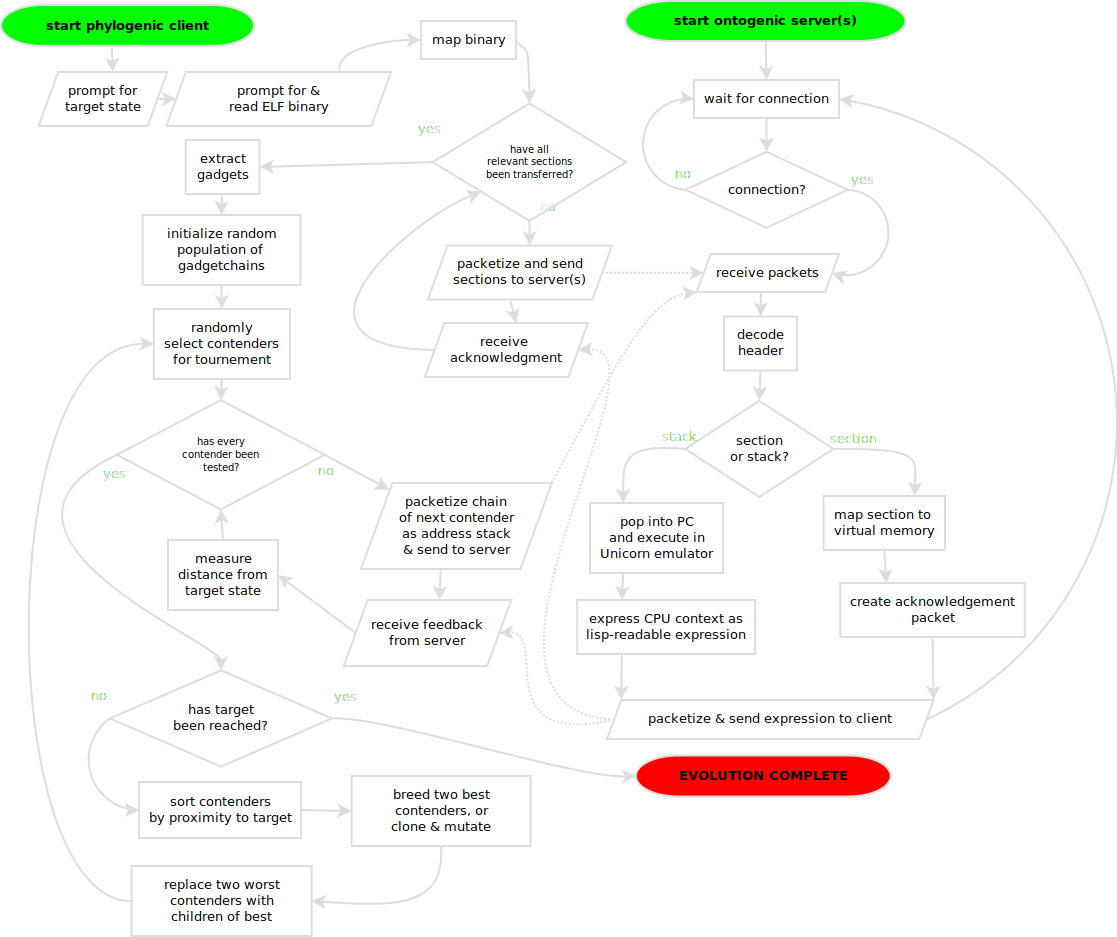
\includegraphics[height=8cm,width=11.5cm]{roper-flow.png} 


\end{frame}




\begin{frame}{0.8 TODO}


\begin{columns}

    \begin{column}{0.3\textwidth}
    
\includegraphics[width=4cm]{inverted-transparent-roper.png}
    \end{column}
    \begin{column}{0.7\textwidth}
    
    \begin{itemize}
    \item ROPER is being designed so as to be easily extensible to other architectures besides 32-bit ARM (x86, x86\_64, MIPS, ARM-64, etc.), so this can and should be actualized;
    \item the tool could be seen as something of a `compiler' for a simple, declarative scripting language. At present this language consists only in simple register patterns, but it could easily be extended into something more `high-level' and useful.
    \item the structure of the tool lends itself well to parallelization and distributed computing, which would increase its efficiency by a few orders of magnitude, if properly implemented.
    \end{itemize} 
    
    \end{column}
\end{columns}
\end{frame}


\begin{frame}
\begin{center}    
    {\huge Progress Report \# 1}
    \vspace{.3cm}
    
    {\large July, 2016}
    \end{center} 
    
\end{frame}

\begin{frame}{1.0: Conceptual Map}

\begin{columns}

\begin{column}{0.5\textwidth}
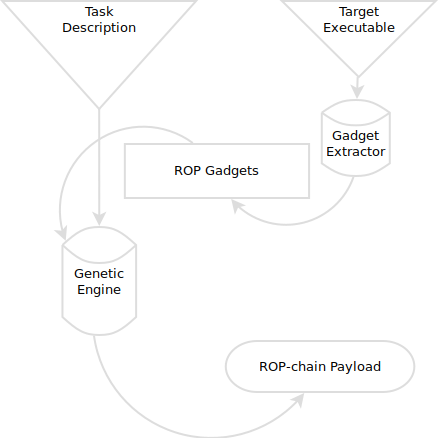
\includegraphics[width=1\textwidth]{simplified.png}

\end{column}

\begin{column}{.5\textwidth}

\begin{itemize}
    \item At a certain level of abstraction, ROPER is just a \emph{compiler}.
    \item It compiles a task description to a ROP-chain,
    \item using the ``gadgets'' extracted from the target as its instruction set
    \item and using a genetic algorithm as its instruction selection algorithm
\end{itemize}

\end{column}

\end{columns}

\end{frame}

\begin{frame}{1.1 Compiler Basics}
\begin{columns}

\begin{column}{0.5\textwidth}
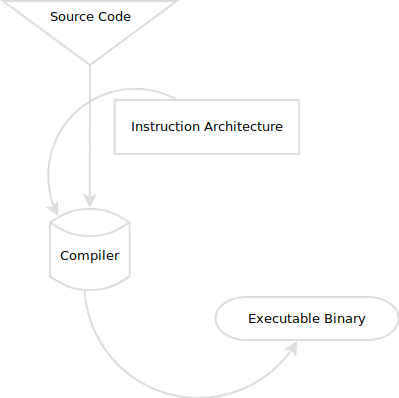
\includegraphics[width=1\textwidth]{compiler.png}

\end{column}
\begin{column}{.5\textwidth}

\begin{itemize}
\item a compiler translates source code to machine code
\item the machine code consists of \emph{instructions} that map onto the primitive actions of the CPU
\item but for ROPER, the primitive ``instructions'' will be the gadgets extracted from the victim binary
\end{itemize}

\end{column}

\end{columns}
\end{frame}
\begin{frame}{1.2 Current State of the Art: Q}

\begin{columns}
\begin{column}{.4\textwidth}


\includegraphics[width=\textwidth]{Q.png}

\end{column}

\begin{column}{.60\textwidth}
\begin{itemize}
\item "Q: Exploit Hardening Made Easy", Usenix Security Symposium, 2011: Schwartz, Avgerinos, \& Brumley
\item \textbf{Q} is a fully deterministic compiler, not driven by machine learning, that uses classical algorithms to compile user-written scripts into ROP-chains, using a given binary
\item quite efficient, produces payloads from binaries $>=$ 20KB (tested on common Unix utilities)
\item targets the x86 architecture, while our focus is the ARM and other embedded/mobile RISC architectures
\item neither binary nor source seem to be publicly available
\item we can build on their design, \& incorporate genetic methods to optimize for \textbf{stealth}
\end{itemize}
\end{column}
\end{columns}
% image: Q from James Bond

\end{frame}
\begin{frame}{1.3 Tactical Deployment of Genetic Methods}

\begin{columns}

\begin{column}{0.5\textwidth}
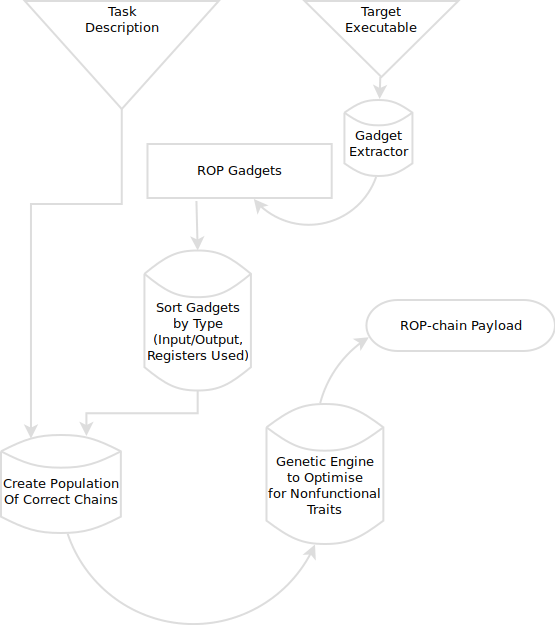
\includegraphics[width=1\textwidth]{less-simple.png}

\end{column}
\begin{column}{.5\textwidth}

\begin{itemize}
\item use efficient deterministic methods wherever applicable
\item we can deterministically compile semantically correct ROP-chains 
\item \textbf{Q} is proof that this can be done
\item we will first design a skeletal, deterministic ROP compiler, \& then exploit genetic methods to optimise for non-semantic properties, like stealth
\item Kayacik's work (in our lab) showed that this, too, is feasible
\end{itemize}

\end{column}

\end{columns}

\end{frame}


\begin{frame}{1.4 Roadmap}
\begin{columns}

\begin{column}{.3\textwidth}
\begin{center}
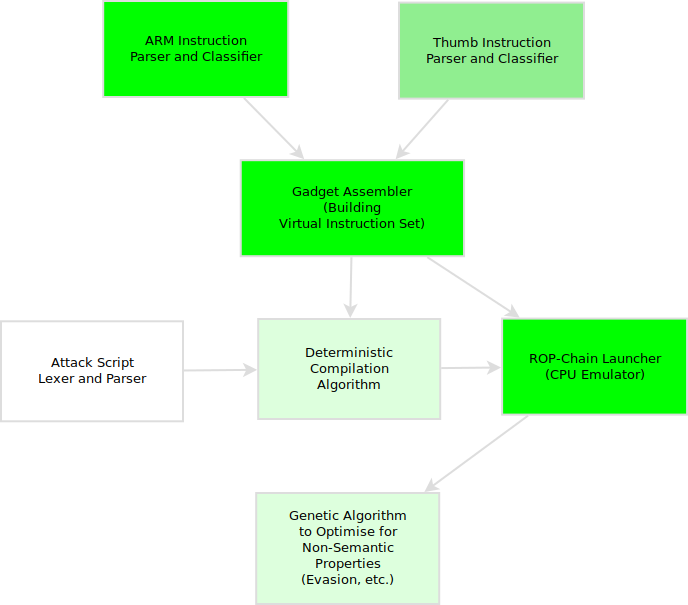
\includegraphics[width=.7\textwidth]{progress.png}
\end{center}
\end{column}

\begin{column}{.7\textwidth}
\begin{itemize}
\item I have ported the gadget-extraction algorithm, which I had earlier written in Lisp, to Haskell, for better integration with the rest of the compiler \& emulator
\item Now working on a type system for the gadgets -- sorting them by input/output, and by registers used, so that they can be easily composed into chains by the deterministic compiling algorithms
\item Planning the genetic components, so as to best take advantage of what they have to offer over and above deterministic compilation algorithms
\item Planning a simple, scheme-like scripting language and parser
\end{itemize}
\end{column}

\end{columns}
\end{frame}



% \begin{frame}{4. Beyond Q}

% \end{frame}

\begin{frame}
\begin{center}    
    {\huge Progress Report \# 2}
    \vspace{.3cm}
    
    {\large August, 2016}
    \end{center} 
    
\end{frame}

\begin{frame}{2.0 Conceptual Map (Recap)}

\begin{columns}

\begin{column}{0.5\textwidth}
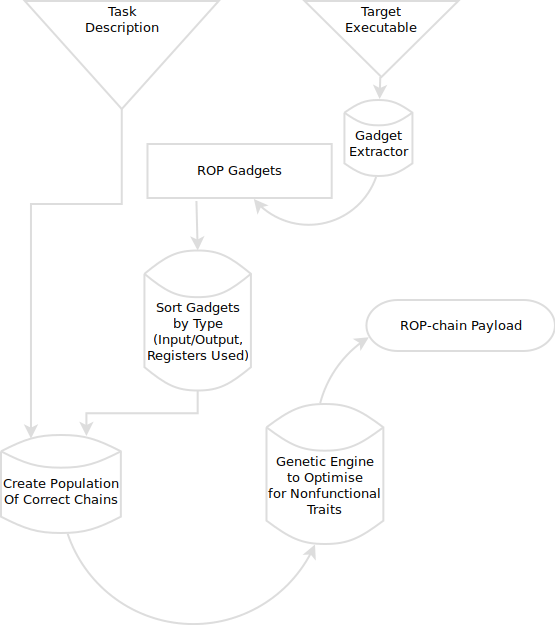
\includegraphics[width=1\textwidth]{less-simple.png}

\end{column}
\begin{column}{.5\textwidth}

\begin{itemize}
\item ROPER is a tool to automatically generate ROP-chains -- exploit payloads that cannibalize a target process's own executable code segment rather than introducing code of their own
\item it hybridizes deterministic compiling techniques with stochastic genetic algorithms
\item the compiler generates an initial population of semantically correct or approximate solutions
\item genetic algorithm optimises for both semantic correctness and non-semantic properties (stealth, brevity, obfuscation, etc.)
\end{itemize}

\end{column}

\end{columns}

\end{frame}


\begin{frame}{2.1 Roadmap}
\begin{columns}

\begin{column}{.3\textwidth}
\begin{center}
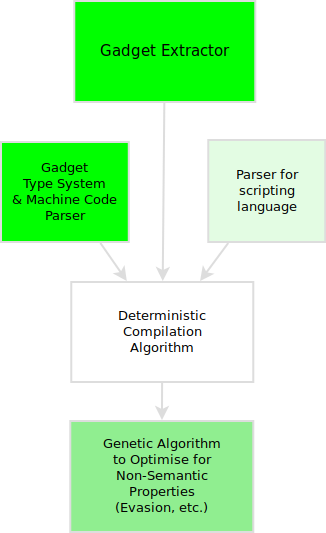
\includegraphics[width=.9\textwidth]{progress2.png}
\end{center}
\end{column}

\begin{column}{.7\textwidth}
\begin{itemize}

\item I am developing a parser that reads compiled ARM machine code, and re-compiles it into series of Haskell functions and data structures.

\item some of this code will be reused in the parser needed to compile the ROPER scripting language into an initial population and directions for the genetic algorithm

\item I've also been experimenting with and prototyping the genetic component, independently of the rest, in LISP and C (with a purely random initial population)

\end{itemize}
\end{column}

\end{columns}
\end{frame}

\begin{frame}{2.2 Parsing and Compiling Machine Code into Haskell Functions}
\begin{columns}
\begin{column}{.5\textwidth}
\begin{itemize}
\item ROPER finds its raw materials (its `instruction architecture') by taking apart a target binary programme
\vspace{1.3cm}
\item it order to process these materials intelligently, it needs to convert them into more tractable structures
\end{itemize}
\end{column}
\begin{column}{.5\textwidth}
\begin{itemize}

\item ROPER partially {decompiles}, or \emph{recompiles}, the binary into a sequence of haskell functions and structures
\vspace{1cm}
\item these can be analyzed and manipulated algebraically, so that they approximate or satisfy the objective given by the user, before being passed to the genetic algorithm
\end{itemize}

\end{column}

\end{columns}
    
\end{frame}

\begin{frame}{2.3 Application of the Type System: Detection of Syntactic Introns}

\begin{columns}

\begin{column}{.5\textwidth}
\includegraphics[width=\textwidth]{"exons.png"}
\end{column}

\begin{column}{.5\textwidth}


`Introns' are pieces of code (`genes') in a sequence that have no semantic or functional effect on its output. Our type system will let us detect and manipulate them.

\begin{itemize}

\item The concept has a biological analogy in `junk DNA'. 

\item Introns confer interesting and useful non-semantic features on the evolving algorithms:

\begin{itemize}
\item[>>] robustness to mutation -- if a mutation affects intron segments, it will not semantically alter the output
\item[>>] punctuated equilibrium -- changes can accumulate for some time before being suddenly `switched on'
\item[>>] potential for obfuscation
\end{itemize}
\end{itemize}
\end{column}

\end{columns}


\end{frame}



\begin{frame}{2.4 Prototyping the Genetic Algorithms in Lisp}

\begin{columns}
\begin{column}{.45\textwidth}
%% \begin{itemize}
%%\item 
While developing the initial population compiler in Haskell, I experimented with a quick and dirty implementation of a few genetic algorithms in Lisp, and an ARM emulator server written in C.

\vspace{.15cm}


%%\item 
The initial population, here, was \emph{entirely randomized}, and the task was relatively simple: 
\vspace{.25cm}
\begin{itemize}
\item[>>] \emph{bring the CPU context to a desired state, specified by a register pattern}
\end{itemize}
\vspace{.25cm}
{\small E.g.  \texttt{\#(0x01 \_ 0x04 \_ \_ \_ 0x05 ) } 
%\_ \_ \_ \_ \_)}\end{itemize}
means: \emph{set R0 to 0x01, R2 to 0x03, and R6 to 0x05}}

\end{column}
\begin{column}{.55\textwidth}
%%\begin{itemize}
Candidate fitness functions:
\begin{itemize}
\item[>>] {\small An adaptation of Lexicase Selection: for each relevant register $R$, in random order, assess each creature in the population, and discard any that fail to correctly set $R$. When two remain, mate them, and replace the first culled with their child.}
\item[>>] {\small A Euclidean distance function: treat the desired register pattern as an $n$-dimensional hyperplane in 15-dimensional space (for 15 registers). A creature's fitness is the distance between the register state it achieves and the target hyperplane.}
\end{itemize}
{\small The second met with greater success: after about 1000 generations, a 32 gadget-long chain emerged that satisfied the test pattern. }
\end{column}
\end{columns}
    
\end{frame}






% \begin{frame}{4. Beyond Q}

% \end{frame}


\begin{frame}
\begin{center}    
    {\huge Progress Report \# 3}
    \vspace{.3cm}
    
    {\large October, 2016}
    \end{center} 
    
\end{frame}

\begin{frame}{3.0 Conceptual Map (Recap)}

\begin{columns}

\begin{column}{0.5\textwidth}
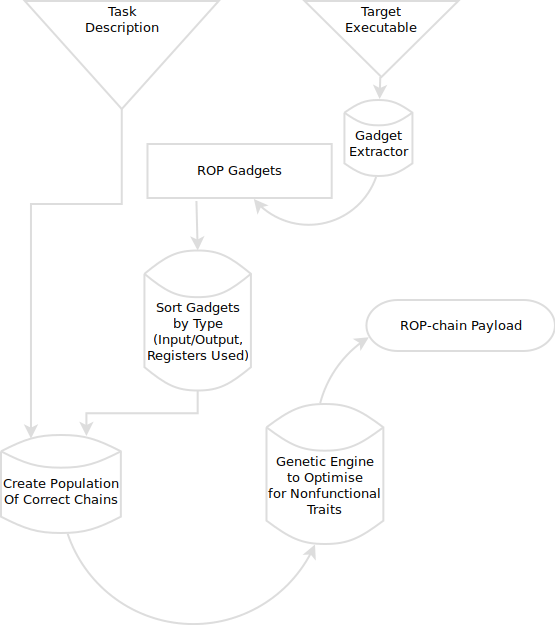
\includegraphics[width=1\textwidth]{less-simple.png}

\end{column}
\begin{column}{.5\textwidth}

\begin{itemize}
\item ROPER is a tool to automatically generate ROP-chains -- exploit payloads that cannibalize a target process's own executable code segment rather than introducing code of their own
\item it hybridizes deterministic compiling techniques with stochastic genetic algorithms
\item the compiler generates an initial population of semantically correct or approximate solutions
\item genetic algorithm optimises for both semantic correctness and non-semantic properties (stealth, brevity, obfuscation, etc.)
\end{itemize}

\end{column}

\end{columns}

\end{frame}


\begin{frame}{3.1 Roadmap}
\begin{columns}

\begin{column}{.4\textwidth}
\begin{center}
\includegraphics[width=\textwidth]{"progress3.png"}
\end{center}
\end{column}

\begin{column}{.6\textwidth}
\begin{itemize}\small
\item Much of the work in the past two months has involved porting the code to Haskell (from Lisp and C) and optimizing its performance.

\item The parsers for binary ARM and Thumb instructions are new, however, and are now complete, facilitating the analysis of compiled machine code.

\item I have rebuilt the emulator responsible for launching ROP chains and reporting on their effects on the CPU context, which is essential for determining their fitness.

\item I have completely redesigned the gadget extractor so that it now takes advantage of the type data synthesized by the instruction parser, better priming the initial population of chains.

\end{itemize}
\end{column}

\end{columns}
\end{frame}

\begin{frame}[fragile]{3.2 Instruction Analysis \& Gadget Synthesis}
\small
\begin{verbatim}
Ok, modules loaded: Gadget, ARMCommon, ARMParser, Aux, ElfHelper, ARM32, Thumb16.
*Gadget> testGadget "data/ldconfig.real" 2
------------------------------------------------------------
[00089018-00089038]: 8 instructions; SP moves 8
------------------------------------------------------------
00089018:  e0030590: ARM Mult --; r0 -> r3 
0008901c:  e0854890: ARM MultLong --; r8 r0 -> r4 r5 
00089020:  e0283198: ARM Mult --; r3 -> r8 
00089024:  e0885005: ARM (DataProc ADD) --; r8 -> r5 
00089028:  e0564004: ARM (DataProc SUB) --; r6 -> r4 
0008902c:  e0c75005: ARM (DataProc SBC) --; r7 -> r5 
00089030:  e1c940f0: ARM HalfWordDataR --; r0 r4 -> r4 
00089034:  e8bd83f8: ARM BlockDataTrans --; r13 -> r3 r4 r5 r6 r7 r8 r9 r15 
------------------------------------------------------------
------------------------------------------------------------
[00088760-00088768]: 2 instructions; SP moves 6
------------------------------------------------------------
00088760:  e1a00005: ARM (DataProc MOV) --; r0 -> r0 
00088764:  e8bd80f8: ARM BlockDataTrans --; r13 -> r3 r4 r5 r6 r7 r15 
------------------------------------------------------------

Number of gadgets: 453
*Gadget> 

\end{verbatim}

    
\end{frame}

\begin{frame}
\begin{center}    
    {\huge Progress Report \# 4}
    \vspace{.3cm}
    
    {\large November, 2016}
    \end{center} 
    
\end{frame}

\begin{frame}{4.1 Roadmap}
\begin{columns}
\begin{column}{.4\textwidth}
\begin{center}
\includegraphics[width=\textwidth]{"progress4.png"}
\end{center}
\end{column}
\begin{column}{.6\textwidth}
\begin{itemize}
\item The emulator is now capable of evaluating not just shellcode, but full ROP-chains. Essential for mapping genotype to phenotype, and determining ``fitness''.
\item A baseline, `low-entropy' compiler is ready -- the worst of all possible proto-compilers -- and generates random ROP-chains with minimal structure, just enough to preserve the integrity of the stack.
\item A crude measure of fitness is now possible, enough to begin the natural-selective process.
\item A simple mating algorithm has been defined, allowing the chains to sexually reproduce.

\end{itemize}
\end{column}
\end{columns}
\end{frame}

\begin{frame}[fragile]{4.2 Random Chains with Stack Integrity}
\small
\begin{verbatim}
------------------------------------------------------------
[0001e818-0001e81b]: 3 instructions; SP moves 8
------------------------------------------------------------
0001e818:  e2844002: ARM (DataProc ADD) #&00000002; r4 -> r4
0001e81c:  e1a00004: ARM (DataProc MOV) --; r0 -> r0
0001e820:  e8bd83f8: ARM (BlockDataTrans LDMFD) --; r13 -> r3 r4 r5 r6 r7 r8 r9 r15
------------------------------------------------------------
,[Immediate: fb89de96]
,[Immediate: 6d3af1d6]
,[Immediate: a9c1796f]
,[Immediate: e2114840]
,[Immediate: 8f45f7aa]
,[Immediate: c21df982]
,[Immediate: 2567d5a6]
,------------------------------------------------------------
[000488f4-000488f6]: 2 instructions; SP moves 6
------------------------------------------------------------
000488f4:  e1a00005: ARM (DataProc MOV) --; r0 -> r0
000488f8:  e8bd81f0: ARM (BlockDataTrans LDMFD) --; r13 -> r4 r5 r6 r7 r8 r15
------------------------------------------------------------
,[Immediate: fb89de96]
,[Immediate: 6d3af1d6]
,[Immediate: a9c1796f]
,[Immediate: e2114840]
,[Immediate: 8f45f7aa]
,------------------------------------------------------------
\end{verbatim}
    
\end{frame}

\begin{frame}[fragile]{4.3 ROP-chain Execution Emulation}

The executable and data sections of the target
binary are mapped into the emulator's virtual
memory. A ROP-chain -- a stack of addresses and
immediate values -- is pushed onto the target's
stack, and then popped into its program counter,
seizing the flow of control.

\tiny
\begin{verbatim}
--| Tracing gadget at 0x0001e818, gadget size = 0x0000000c
    0001e818: e2844002
r0:  00000000  r1:  00000000  r2:  00000000  r3:  00000000  r4:  00000000  r5:  00000000  r6:  00000000  r7:  00000000
r8:  00000000  r9:  00000000  r10: 00000000  r11: 00000000  r12: 00000000  r13: 000b423c  r14: 00000000  r15: 0001e818
    0001e81c: e1a00004
r0:  00000000  r1:  00000000  r2:  00000000  r3:  00000000  r4:  00000002  r5:  00000000  r6:  00000000  r7:  00000000
r8:  00000000  r9:  00000000  r10: 00000000  r11: 00000000  r12: 00000000  r13: 000b423c  r14: 00000000  r15: 0001e81c
    0001e820: e8bd83f8
r0:  00000002  r1:  00000000  r2:  00000000  r3:  00000000  r4:  00000002  r5:  00000000  r6:  00000000  r7:  00000000
r8:  00000000  r9:  00000000  r10: 00000000  r11: 00000000  r12: 00000000  r13: 000b423c  r14: 00000000  r15: 0001e820

--| Tracing gadget at 0x000488f4, gadget size = 0x00000008
    000488f4: e1a00005
r0:  00000002  r1:  00000000  r2:  00000000  r3:  fb89de96  r4:  6d3af1d6  r5:  a9c1796f  r6:  e2114840  r7:  8f45f7aa
r8:  c21df982  r9:  2567d5a6  r10: 00000000  r11: 00000000  r12: 00000000  r13: 000b425c  r14: 00000000  r15: 000488f4
    000488f8: e8bd81f0
r0:  a9c1796f  r1:  00000000  r2:  00000000  r3:  fb89de96  r4:  6d3af1d6  r5:  a9c1796f  r6:  e2114840  r7:  8f45f7aa
r8:  c21df982  r9:  2567d5a6  r10: 00000000  r11: 00000000  r12: 00000000  r13: 000b425c  r14: 00000000  r15: 000488f8
\end{verbatim}
\end{frame}

\begin{frame}[fragile]{4.4 Preliminary Sketch of Fitness Evaluation}
This already gives us enough for a crude calculation of ``fitness'' -- a measure of how closely the CPU context resulting from the chain approximates our
target context. 
\small
\begin{verbatim}
  type Goal = ([Int], [Int])
 
  goal :: Goal
  goal = ([0, 1, 12], [100, 2, 0xdeadbeef])
 
  distance :: Goal -> [Int] -> Int
  distance (idxs,target) out =
    let focus = map (out !!) idxs
    in  sum $ map abs $ zipWith (-) focus target
 
  evalChain :: Emulator Engine -> [Gadget] -> IO Int
  evalChain uc chain =
    (distance goal . take 16) <$> hatchChain uc (unicornPack chain)
\end{verbatim}
\normal

But we can get a much more fine-grained picture as well, and measure things like error-proneness, efficiency, contents of dereferenced pointers (and not just immediate values), etc., which our emulator makes readily available.

\end{frame}

\begin{frame}[fragile]{4.5 Groundwork for Reproduction}
This (very tweakable) fitness functions gives us a basis for probabilistically choosing `parents' for each subsequent generation of chains. Two chains (lists of gadgets) can be mated using a simple function:
\small
\begin{verbatim}
   mate :: RandomGen g => Chain -> Chain -> Rand g Chain
   mate mom dad = (++) <$> flip take mom <*> flip drop dad <$> pivot
     where pivot = getRandomR (0, length mom - 1)
\end{verbatim}
\normal
which splices the two parent chains together, at a random index, to create a child.

The next block of work on this project will be 
\begin{enumerate} 
\item to 
fine-tune the selection, reproduction, and mutation
algorithms, while
\item refining the functions responsible for preparing the initial population of chains (the deterministic compiler algorithms)
\end{enumerate}
\end{frame}

\begin{frame}
\begin{center}    
    {\huge Progress Report \# 5}
    \vspace{.3cm}
    
    {\large January, 2017}
    \end{center} 
    
\end{frame}

\begin{frame}{5.0 The Trouble with Sexual Reproduction}
\begin{itemize}
\item we want a way to combine \emph{partial} solutions and useful discoveries -- ``building blocks'' -- into more complete solutions,
\item sexual reproduction, or ``crossover'', is an attempt to do just this

\end{itemize}
\begin{tabular}{c|c}
 \includegraphics[width=.5\textwidth]{"steamboat.png"}    &  \includegraphics[width=.4\textwidth]{"CarDiagram.jpg"}
\end{tabular}
%\begin{center}
%\includegraphics[width=.5\textwidth]{%"car-boat-crossover-mess.jpg"}
%\end{center}
    
\end{frame}

\begin{frame}{5.1 The Trouble with Sexual Reproduction}

\begin{tabular}{c|c}
 \includegraphics[width=.5\textwidth]{"steamboat.png"}    &  \includegraphics[width=.4\textwidth]{"CarDiagram.jpg"}
\end{tabular}
\begin{center}
\includegraphics[width=.5\textwidth]{"car-boat-crossover-mess.jpg"}
\end{center}

\begin{itemize}
\item \dots but nothing insures that crossover will cut the genome at the joints
\item more often than not, the results will be chaotic, and destructive of any ``building blocks'' formed.
\end{itemize}

\end{frame}

\begin{frame}{5.2 The Trouble with Sexual Reproduction}

\begin{tabular}{c|c}
 \includegraphics[width=.5\textwidth]{"steamboat.png"}    &  \includegraphics[width=.4\textwidth]{"CarDiagram.jpg"}
\end{tabular}
\begin{center}
\includegraphics[width=.5\textwidth]{"car-boat-crossover.jpg"}
\end{center}

\begin{itemize}
\item What we want is a mechanism that will \emph{predispose} crossover towards preserving building blocks and adaptive gene linkages,
\item and since we can't know in advance what the building blocks will be, this mechanism needs to be emergent.
\end{itemize}
    
\end{frame}

\begin{frame}{5.3 ROPER's approach to the problem}


\begin{itemize}
    \item The basic intuition, here, is that genes that tend to occur side-by-side in relatively fit individuals are likely to be genes that should continue to ``stick'' together.
    \item This is reflected in a ``viscosity'' field, which is attached to each gene. The higher the viscosity, the less likely the neighbouring genes are to be separated by a crossover event.
    \item We can either make the viscosity value strictly correlative to fitness patterns, or subject it to slow mutation as well.
\end{itemize}

\begin{center}
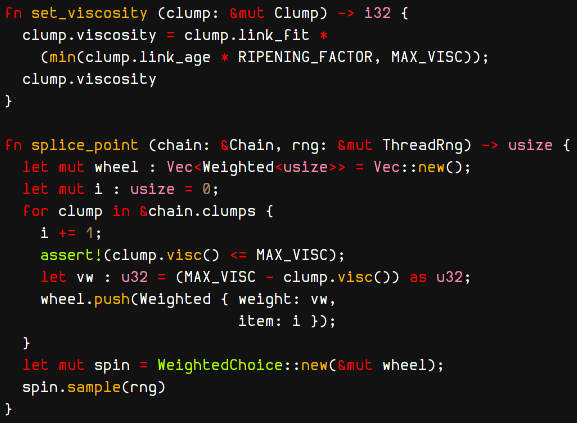
\includegraphics[width=.6\textwidth]{splice_point.png}
\end{center}

\end{frame}

\begin{frame}{5.4 Representation of the ROP-Chain Genome in ROPER}
\begin{columns}



\begin{column}{0.6\textwidth}
    
\begin{itemize}
    \item I've also changed the representation of the genome in ROPER, building on the stack integrity mechanisms introduced in the last report. 
    
    \item The basic unit used in crossover is no longer a single 32-bit word (the address of a gadget or an immediate value), but a `clump' consisting of a gadget address, followed by a series of immediate values that that gadget will pop from the stack. 
    
    \item An executable payload is composed by overlapping the clumps like shingles, ensuring that each clump will pop an executable address into the program counter (PC) register when it returns.
    \end{itemize}
    \end{column}
\begin{column}{0.4\textwidth}
    
\includegraphics[width=\textwidth]{clumps.png}
\end{column}
\end{columns}


\end{frame}

\begin{frame}{5.5 Crossover and Mutation Operators}


\begin{itemize}
    \item Crossover operates only on `clumps', and the choice of crossover site is influenced by the clumps' viscosity fields.

    \item  Mutation operates inside each clump, and alters the immediate values either through arithmetical operations, permutation, or indirection -- searching for occurrences of similar values in the target binary, and replacing the value with a pointer to one of those occurrences.
\end{itemize}
\end{frame}

\begin{frame}{5.6 Next}

\begin{itemize}
    \item The platform is nearly ready to begin full-fledged evolutionary runs -- it's just a matter of writing a bit of glue code to combine the various modules developed so far, namely:
    
    \begin{itemize}
        \item the ARMv7 CPU emulator interface, responsible for genotype $\rightarrow$ phenotype mapping (ontogenesis),
        \item the ARM and THUMB binary analysis modules, and gadget extractors
        \item the sexual reproduction (crossover) and mutation algorithms, and
        \item the selection algorithm (tournement), which combined with the mutation and reproduction operators form the phylogenetic component of the system,
        \item the fitness function, currently implemented as a vectorial distance measure modified by penalties for runtime errors
    \end{itemize}
    
    \item Once these are combined, we can begin experimenting with different fitness functions, tweaks to the reproduction and variation operators, optimisations, and so on. 
    \item Preliminary quantitative results should be available by the time we next meet. 
\end{itemize}


\end{frame}

\end{document}
